%----------------------------------------------------------------------------------------
%	PACKAGES AND OTHER DOCUMENT CONFIGURATIONS
%----------------------------------------------------------------------------------------

\documentclass[paper=a4, fontsize=11pt]{scrartcl} % A4 paper and 11pt font size
\usepackage{multicol}
\usepackage[T1]{fontenc} % Use 8-bit encoding that has 256 glyphs
\usepackage{fourier} % Use the Adobe Utopia font for the document - comment this line to return to the LaTeX default
\usepackage[english]{babel} % English language/hyphenation
\usepackage{amsmath,amsfonts,amsthm} % Math packages
\usepackage{listings}
\usepackage{lipsum} % Used for inserting dummy 'Lorem ipsum' text into the template
\usepackage{graphicx}
\usepackage{subfig}

\usepackage{sectsty} % Allows customizing section commands
\allsectionsfont{\centering \normalfont\scshape} % Make all sections centered, the default font and small caps

\usepackage{fancyhdr} % Custom headers and footers
\pagestyle{fancyplain} % Makes all pages in the document conform to the custom headers and footers
\fancyhead{} % No page header - if you want one, create it in the same way as the footers below
\fancyfoot[L]{} % Empty left footer
\fancyfoot[C]{} % Empty center footer
\fancyfoot[R]{\thepage} % Page numbering for right footer
\renewcommand{\headrulewidth}{0pt} % Remove header underlines
\renewcommand{\footrulewidth}{0pt} % Remove footer underlines
\setlength{\headheight}{13.6pt} % Customize the height of the header

%\numberwithin{equation}{section} % Number equations within sections (i.e. 1.1, 1.2, 2.1, 2.2 instead of 1, 2, 3, 4)
%\numberwithin{figure}{section} % Number figures within sections (i.e. 1.1, 1.2, 2.1, 2.2 instead of 1, 2, 3, 4)
%\numberwithin{table}{section} % Number tables within sections (i.e. 1.1, 1.2, 2.1, 2.2 instead of 1, 2, 3, 4)

%\setlength\parindent{0pt} % Removes all indentation from paragraphs - comment this line for an assignment with lots of text

%----------------------------------------------------------------------------------------
%	TITLE SECTION
%----------------------------------------------------------------------------------------

\newcommand{\horrule}[1]{\rule{\linewidth}{#1}} % Create horizontal rule command with 1 argument of height

\title{	
\normalfont \normalsize 
\textsc{Syddansk Universitet} \\ [25pt] 
\horrule{0.5pt} \\[0.4cm] % Thin top horizontal rule
\huge Data Preprocessing \\ % The assignment title
\horrule{2pt} \\[0.5cm] % Thick bottom horizontal rule
}

\author{Bjarki Sigurdsson \\ Abdulrahman Abdulrahim \\ Miguel de la Colina}
 % Your name

\date{\normalsize\today} % Today's date or a custom date

\begin{document}

\maketitle % Print the title

%----------------------------------------------------------------------------------------
%	PROBLEM 1
%----------------------------------------------------------------------------------------


\section*{Abstract}

\paragraph{The purpose of the exercise was to examine the effects of preprocessing on kNN classification. We specifically tested Principal Component Analysis (PCA) and Min-Max Normalization. Other preprocessing methods used were those provided in the previous exercise by the \texttt{loadimage.r} script, namely image smoothing and DPI downsampling.}
%The purpose of this report is to use the k-nearest neighbor algorithm on a data-set made of ciphers. We will be dividing the data into two sets, one for training and one for testing. We will analyze the results for different values of k and DPI to see how this alters our results. Also we will be applying the  Gaussian smoothing with various sigmas in order to see how does this alter the results.}  

%------------------------------------------------


%----------------------------------------------------------------------------------------
%	PROBLEM 2
%----------------------------------------------------------------------------------------

\section{PCA}
For this part of the exercise we used PCA to reduce the dimensionality of the data and observed the effect on kNN classification of using the first principal components resembling 80, 90, 95 and 99\% of the total variance. We tested for classification accuracy and computation times for varying k.\par% We refer to the number of principal components used as \#PC.\par
\subsection{Single-person data}
Information on the first 10 principal components, in order, is shown in table \ref{tab:pca}. These correspond to the data from member 1 in group 5. This is how we determine the breakpoints for 80, 90, 95 and 99\% of the total variance. They are 13, 23, 36 and 77, respectively. This is also illustrated in figure \ref{fig:scree}. \par

\begin{table}[h]
\centering
\caption{The first 10 principal components.}
\label{tab:pca}
\begin{tabular}{|c|r|r|r|}
\hline
PC\# & Standard Deviation & Proportion of Variance & Cumulative PV \\ \hline
1    & .7646              & .1876                  & .1876         \\
2    & .6878              & .1518                  & .3994         \\
3    & .6365              & .1300                  & .4695         \\
4    & .4804              & .0741                  & .5435         \\
5    & .4290              & .0591                  & .6026         \\
6    & .3723              & .0445                  & .6471         \\
7    & .3162              & .0321                  & .6791         \\
8    & .2864              & .0263                  & .7055         \\
9    & .2689              & .0232                  & .7287         \\
10   & .2662              & .0228                  & .7514         \\ \hline
\end{tabular}
\end{table}

\begin{figure}[h]
	\centering
	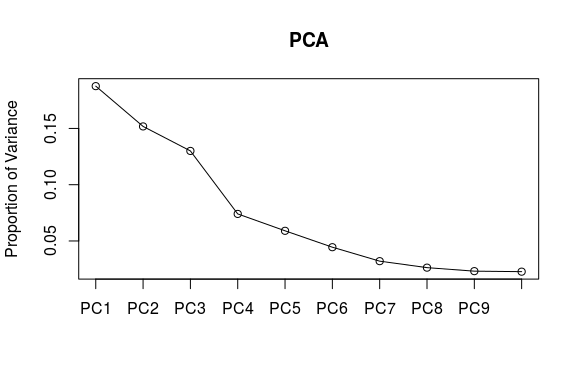
\includegraphics[width=0.8\textwidth]{scree.png}
	\caption{Scree-plot of the first 10 principal components.}
	\label{fig:scree}
\end{figure}

Figure \ref{fig:timing} shows the results from setting k to 50, varying the number of principal components according to the breakpoints mentioned and measuring the average execution time of the kNN classification step. We see that there is a linear relationship between the two.\par

\begin{figure}[h]
	\centering
	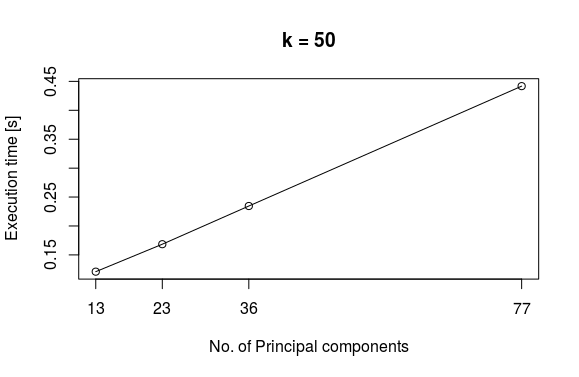
\includegraphics[width=0.8\textwidth]{timing.png}
	\caption{Timing results with a varying number of principal components.}
	\label{fig:timing}
\end{figure}

Figure \ref{fig:acc} shows the classification accuracy for varying numbers of principal components and varying k. We see that the behaviour is similar for varying k and that the effect of using more principal components is negligible above 90\% of total variance.

\begin{figure}[h]
	\centering
	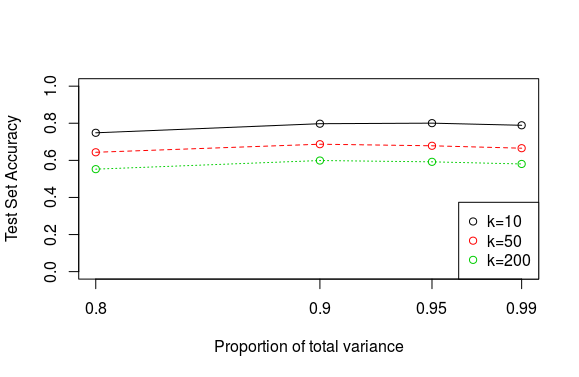
\includegraphics[width=0.8\textwidth]{accuracy2.png}
	\caption{Classification accuracy results for varying k and Proportion of Variance.}
	\label{fig:acc}
\end{figure}

\clearpage
\subsection{Multi-person data}

Information on the first 10 principal components, in order, is shown in table \ref{tab:pca_m}. In this case the breakpoints are 20, 31, 45 and 89 for 80, 90, 95 and 99\%, respectively. This is illustrated in figure \ref{fig:scree_m}.\par

\begin{table}[h]
\centering
\caption{The first 10 principal components.}
\label{tab:pca_m}
\begin{tabular}{|c|r|r|r|}
\hline
PC\# & Standard Deviation & Proportion of Variance & Cumulative PV \\ \hline
1    & .8013              & .1336                  & .1336         \\
2    & .7457              & .1157                  & .2493         \\
3    & .5915              & .0728                  & .3220         \\
4    & .5542              & .0639                  & .3859         \\
5    & .5369              & .0600                  & .4459         \\
6    & .4652              & .0450                  & .4909         \\
7    & .4434              & .0409                  & .5318         \\
8    & .4335              & .0391                  & .5709         \\
9    & .3806              & .0301                  & .6010         \\
10   & .3757              & .0294                  & .6304         \\ \hline
\end{tabular}
\end{table}

\begin{figure}[h]
	\centering
	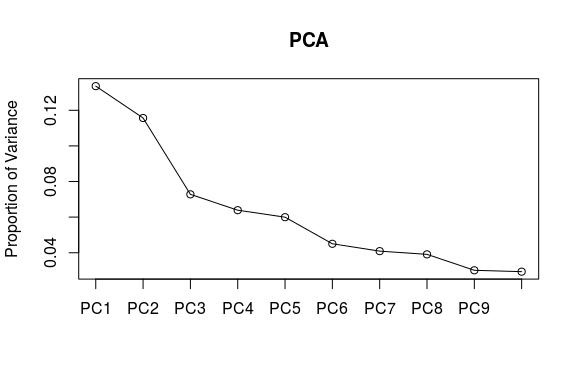
\includegraphics[width=0.8\textwidth]{scree_m.png}
	\caption{Scree-plot of the first 10 principal components.}
	\label{fig:scree_m}
\end{figure}

Figure \ref{fig:timing_m} shows the results from setting k to 50, varying the number of principal components according to the breakpoints mentioned and measuring the average execution time of the kNN classification step. Again we see that there is a linear relationship between the two. This time around the timings were less accurate due to time constraints and the size of the dataset.\par

\begin{figure}[h]
	\centering
	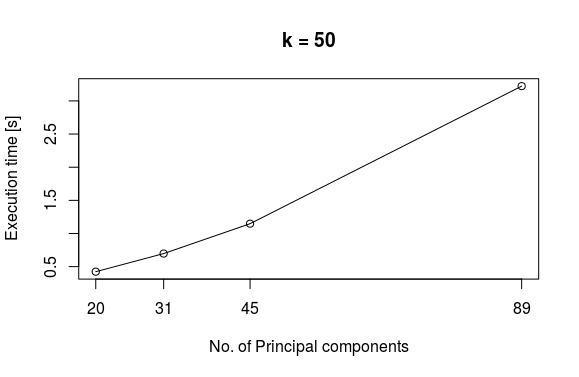
\includegraphics[width=0.8\textwidth]{timing_m.png}
	\caption{Timing results with a varying number of principal components.}
	\label{fig:timing_m}
\end{figure}

Figure \ref{fig:acc_m} shows the classification accuracy for varying numbers of principal components and varying k. This is similar to what we saw for the single-person dataset.%We see that the behaviour is similar for varying k and that the effect of using more principal components is negligible above 90\% of total variance.

\begin{figure}[h]
	\centering
	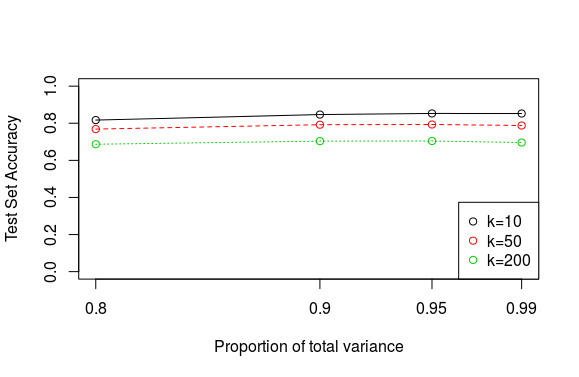
\includegraphics[width=0.8\textwidth]{accuracy2_m.png}
	\caption{Classification accuracy results for varying k and Proportion of Variance.}
	\label{fig:acc_m}
\end{figure}

\clearpage
\section{Normalization}
In this section we analyze the effects of applying Min-Max Normalization before the PCA step (pre-normalization) or after (post-normalization). To this end, we perform a cross-validation of the kNN classifier and compare the results.\par

\subsection{Single-person data}
Figure \ref{fig:hist} shows the results of cross-validation on pre-normalized and post-normalized data. We see that the results are near-identical. This is logical as PCA depends on the eigenvalue decomposition of the covariance matrix and is therefore not significantly altered by normalization via robust methods.

\begin{figure}[h]
    \centering
    \subfloat[Pre-normalization]
	{
        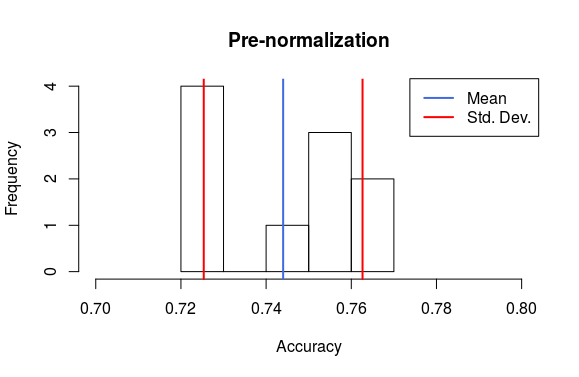
\includegraphics[width=0.49\textwidth]{prenorm.png}
        \label{fig:pre}
	}
	\subfloat[Post-normalization]
	{
        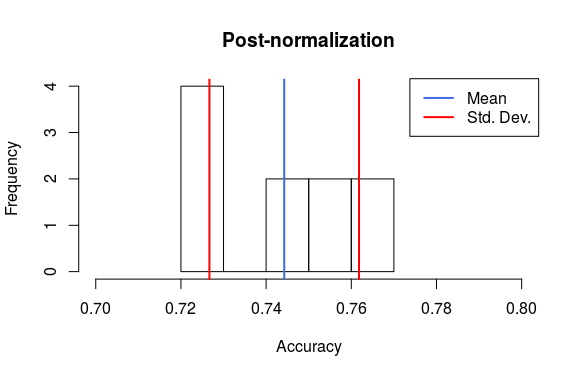
\includegraphics[width=0.49\textwidth]{postnorm.png}
        \label{fig:post}
    }
    \caption{Histogram of cross-validation results with k=50 using 36 principal components (95\% of total variance).}
    \label{fig:hist}
\end{figure}

<<<<<<< HEAD
\clearpage
\subsection{Multi-person data}

Figure \ref{fig:hist} shows the results of cross-validation on pre-normalized and post-normalized data. Again the results are near-identical.%We see that the results are near-identical. This is logical as PCA depends on the eigenvalue decomposition of the covariance matrix and is therefore not significantly altered by normalization via robust methods.

\begin{figure}[h]
    \centering
    \subfloat[Pre-normalization]
	{
        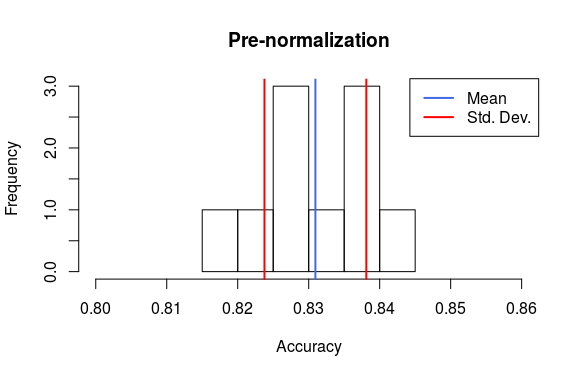
\includegraphics[width=0.49\textwidth]{pre_m.png}
        \label{fig:pre_m}
	}
	\subfloat[Post-normalization]
	{
        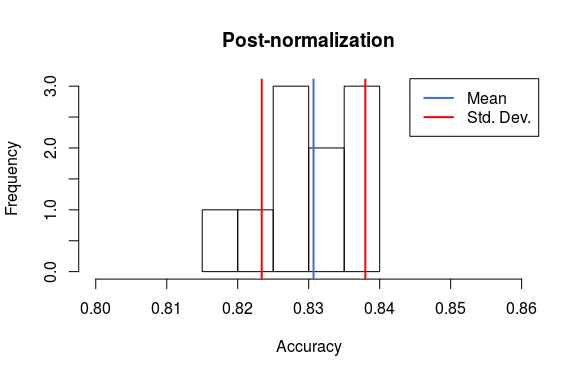
\includegraphics[width=0.49\textwidth]{post_m.png}
        \label{fig:post_m}
    }
    \caption{Histogram of cross-validation results with k=50 using 45 principal components (95\% of total variance).}
    \label{fig:hist_m}
\end{figure}
=======
%------------------------------------------------


%----------------------------------------------------------------------------------------
%	PROBLEM 3
%----------------------------------------------------------------------------------------

\section{Reconstruction}
In this section we will be using the eigenvectors that we got from through PCA in order to reconstruct the images and compare them to the original ciphers. So first we plotted an image of each one of the original ciphers as we can see in figure 4 and figure 5.
\begin{figure}[h]
    \centering
    \subfloat[Cipher 9]
	{
        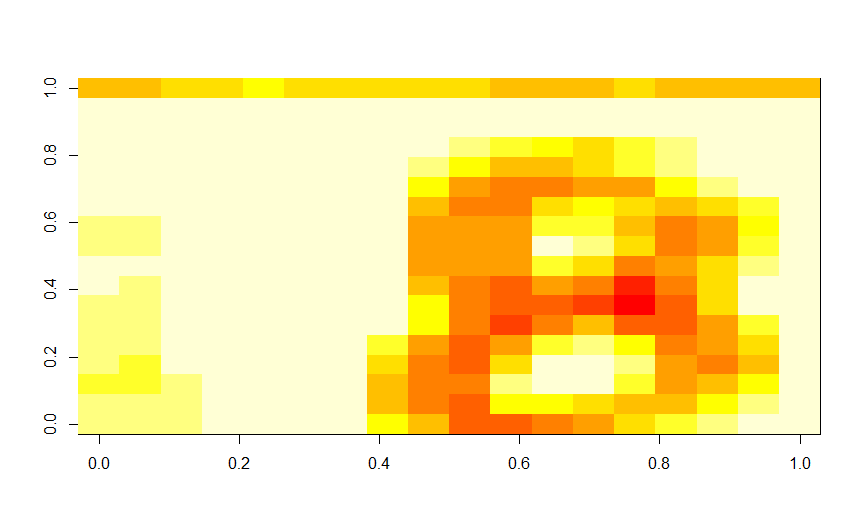
\includegraphics[width=0.49\textwidth]{cipher9.png}
        \label{fig:pre}
	}
	\subfloat[Cipher 10]
	{
        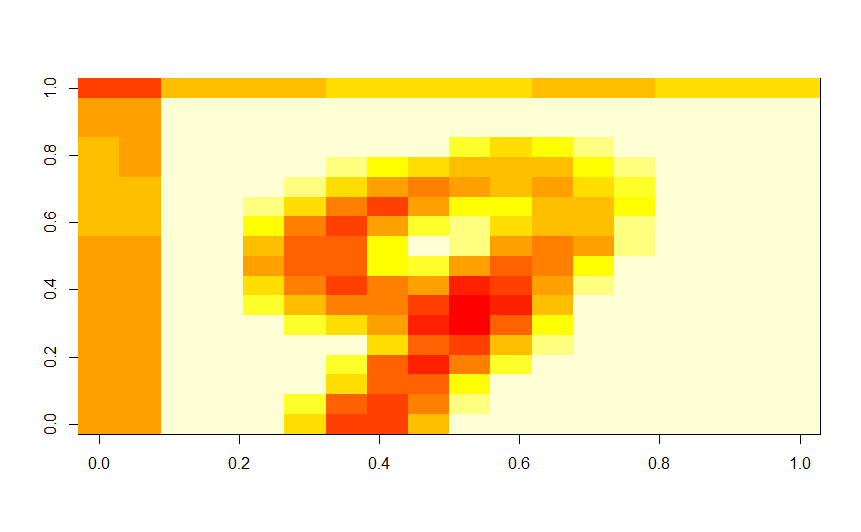
\includegraphics[width=0.49\textwidth]{cipher10.png}
        \label{fig:post}
    }\\
    
    \caption{Original ciphers.}
    \label{fig:ciph}
\end{figure}
\begin{figure}[h]
    \centering
    \subfloat[Cipher 1]
	{
        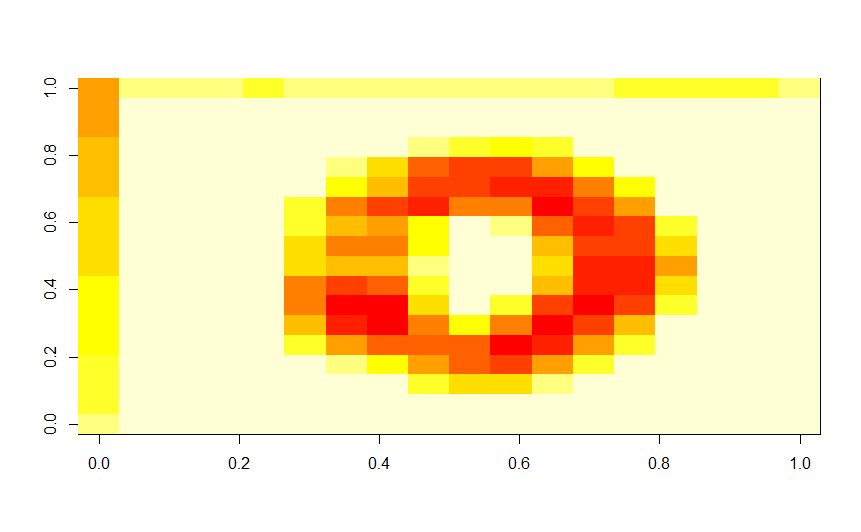
\includegraphics[width=0.49\textwidth]{cipher1.png}
        \label{fig:pre}
	}
	\subfloat[Cipher 2]
	{
        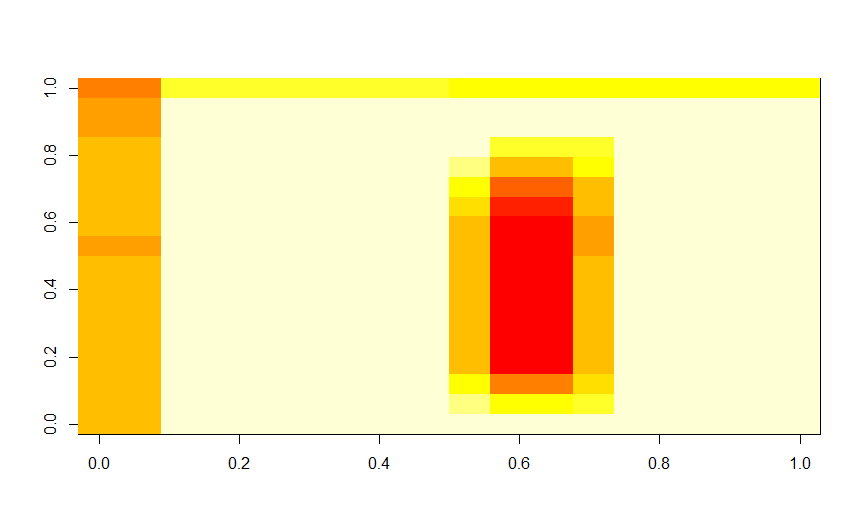
\includegraphics[width=0.49\textwidth]{cipher2.png}
        \label{fig:post}
    }\\
    \subfloat[Cipher 3]
    {
    	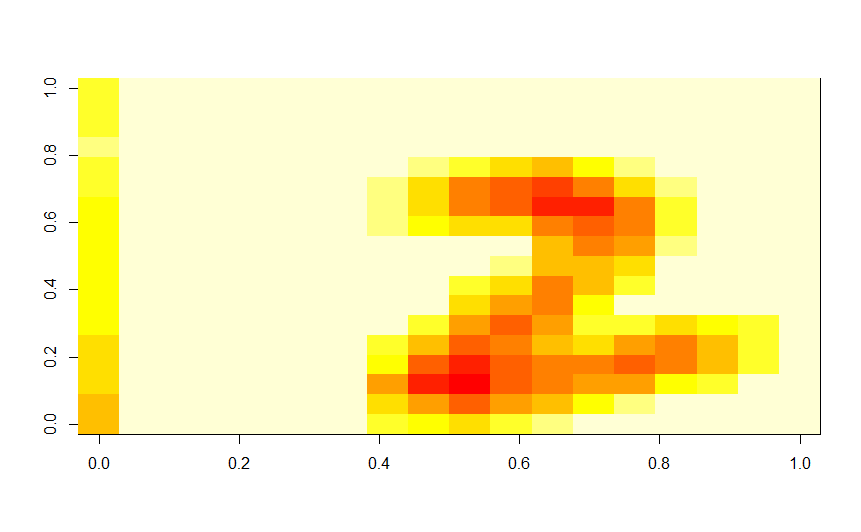
\includegraphics[width=0.49\textwidth]{cipher3.png}
        \label{fig:post}
    }
     \subfloat[Cipher 4]
    {
    	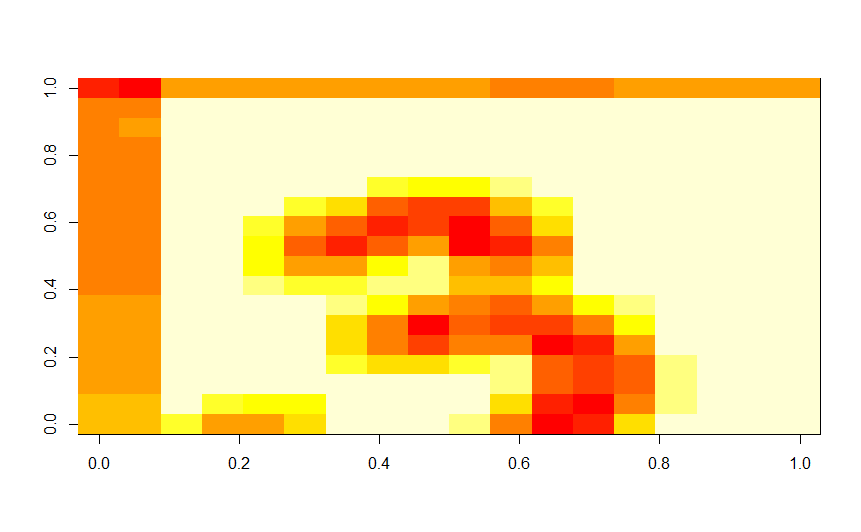
\includegraphics[width=0.49\textwidth]{cipher4.png}
        \label{fig:post}
    }\\
     \subfloat[Cipher 5]
    {
    	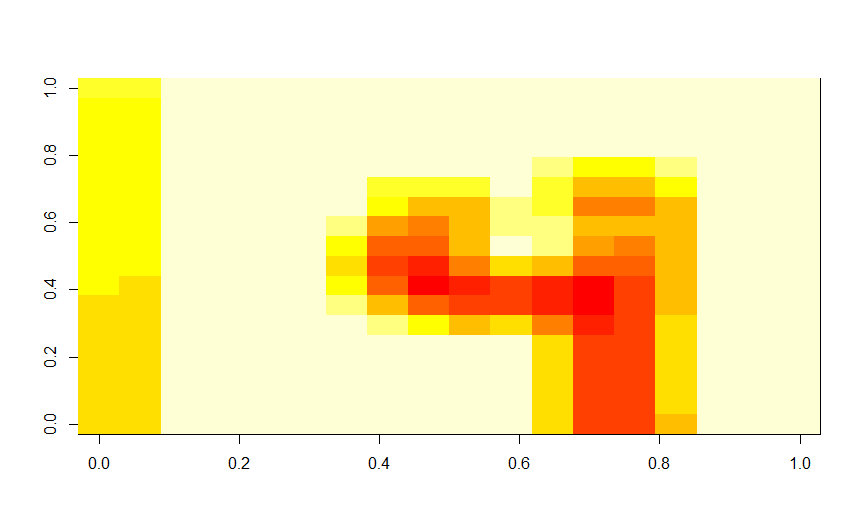
\includegraphics[width=0.49\textwidth]{cipher5.png}
        \label{fig:post}
    }
     \subfloat[Cipher 6]
    {
    	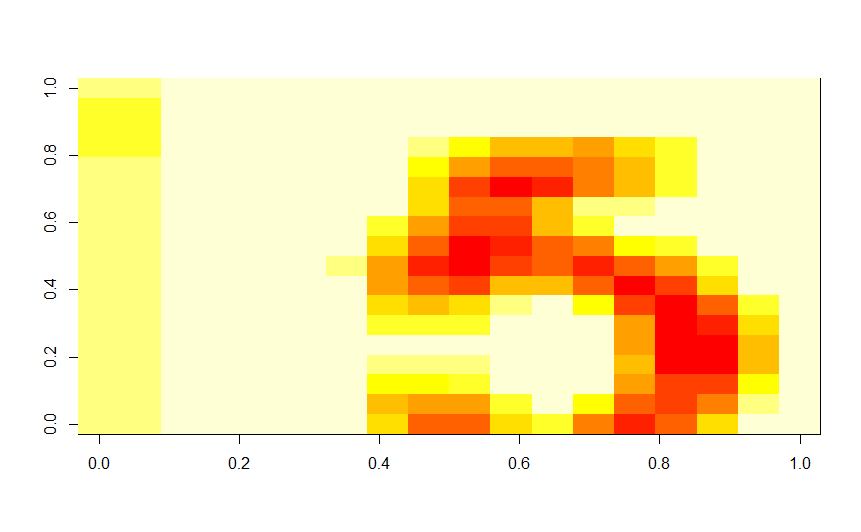
\includegraphics[width=0.49\textwidth]{cipher6.png}
        \label{fig:post}
    }\\
     \subfloat[Cipher 7]
    {
    	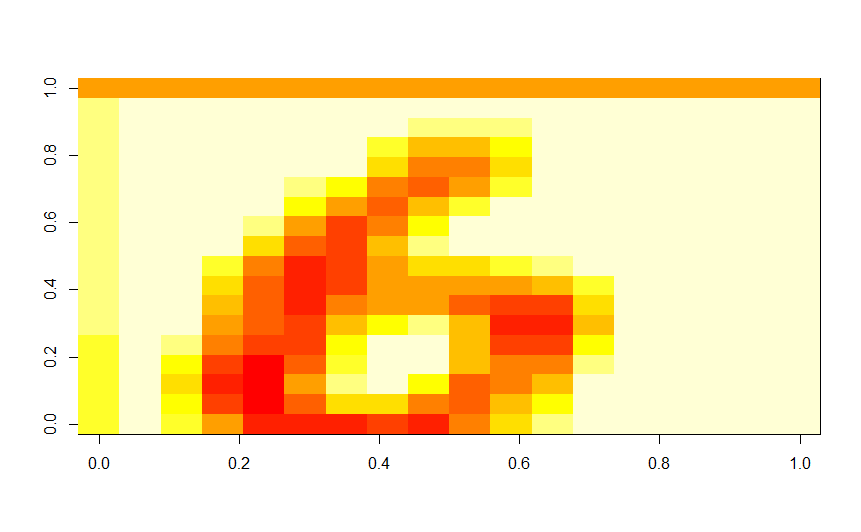
\includegraphics[width=0.49\textwidth]{cipher7.png}
        \label{fig:post}
    }
     \subfloat[Cipher 8]
    {
    	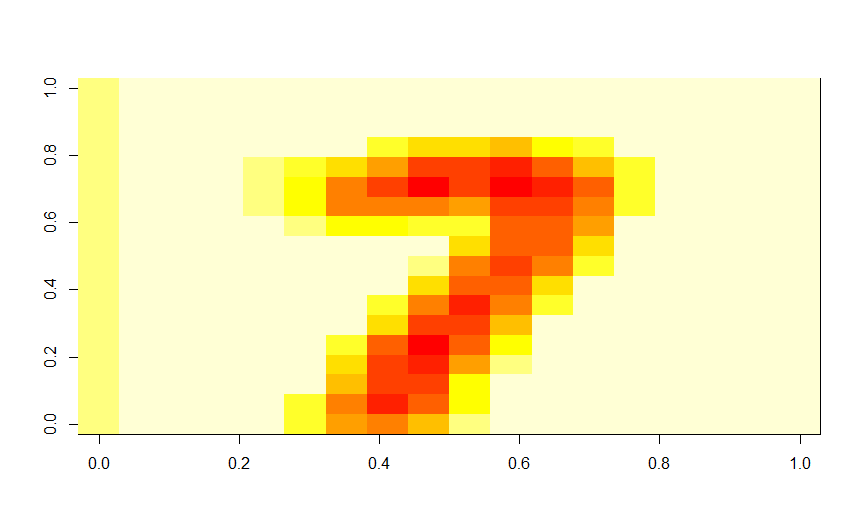
\includegraphics[width=0.49\textwidth]{cipher8.png}
        \label{fig:post}
    }    
    \caption{Original ciphers.}
    \label{fig:ciph}
\end{figure}
\clearpage




\subsection{Eigenvectors}
Then we plotted the first 10 eigenvectors that we got from running the pca algorithm through our original data set as we can see in figure 6 and 7. What we can see when we look at the eigenvectors is high pixel values in areas that have high variances 

\begin{figure}[h]
    \centering
    \subfloat[Eigenvector 1]
	{
        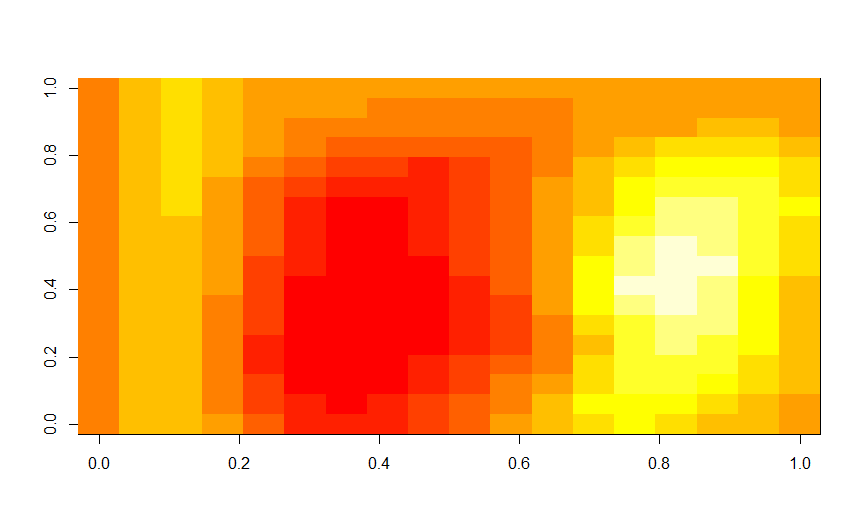
\includegraphics[width=0.49\textwidth]{eigen1.png}
        \label{fig:pre}
	}
	\subfloat[Eigenvector 2]
	{
        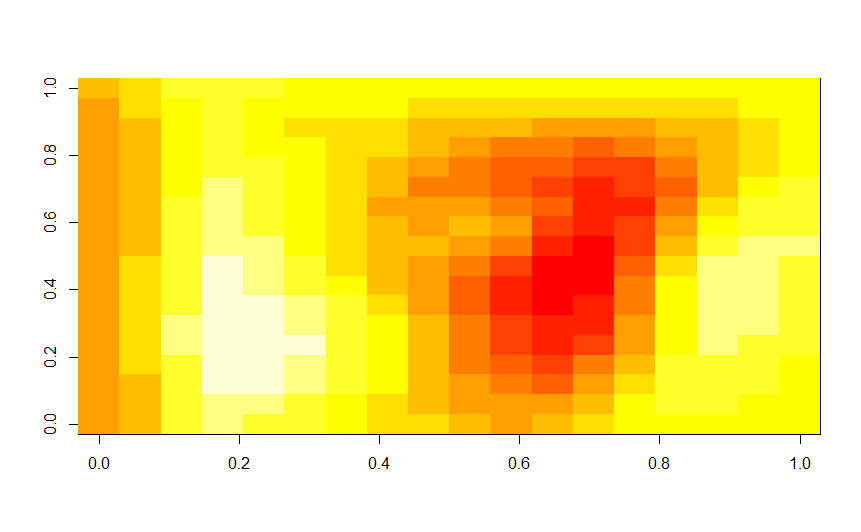
\includegraphics[width=0.49\textwidth]{eigen2.png}
        \label{fig:post}
    }\\
    \subfloat[Eigenvector 3]
    {
    	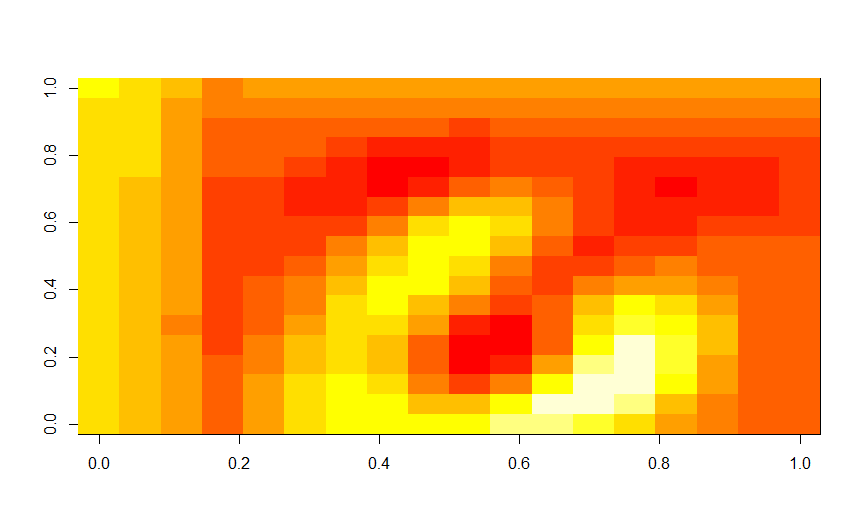
\includegraphics[width=0.49\textwidth]{eigen3.png}
        \label{fig:post}
    }
     \subfloat[Eigenvector 4]
    {
    	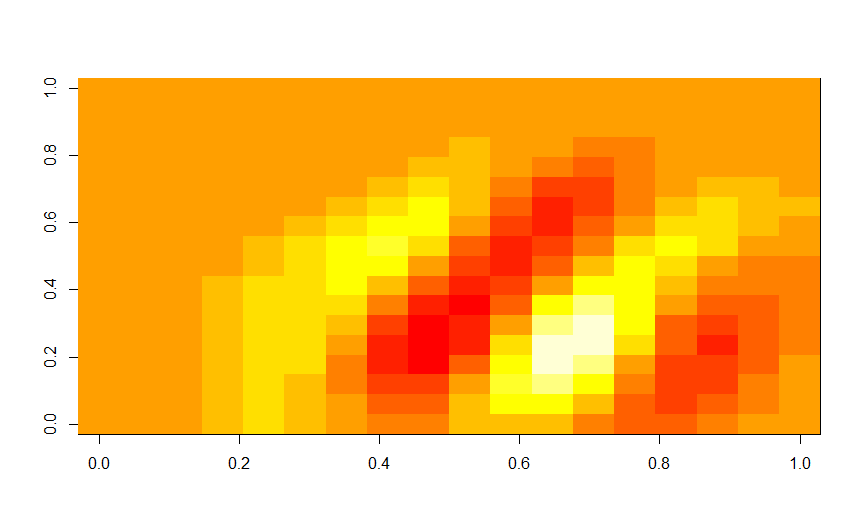
\includegraphics[width=0.49\textwidth]{eigen4.png}
        \label{fig:post}
    }\\ 
    \caption{Eigenvectors}
    \label{fig:hist}
\end{figure}
\begin{figure}[h]
    \centering
     \subfloat[Eigenvector 5]
    {
    	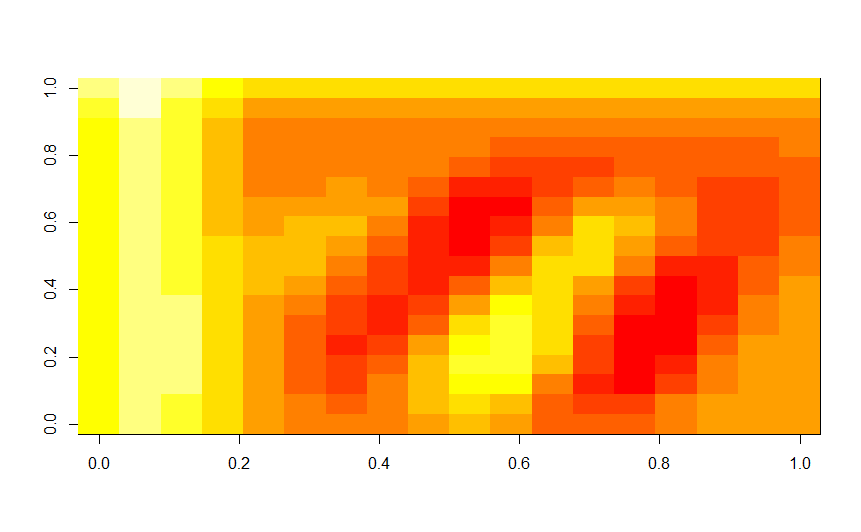
\includegraphics[width=0.49\textwidth]{eigen5.png}
        \label{fig:post}
    }
     \subfloat[Eigenvector 6]
    {
    	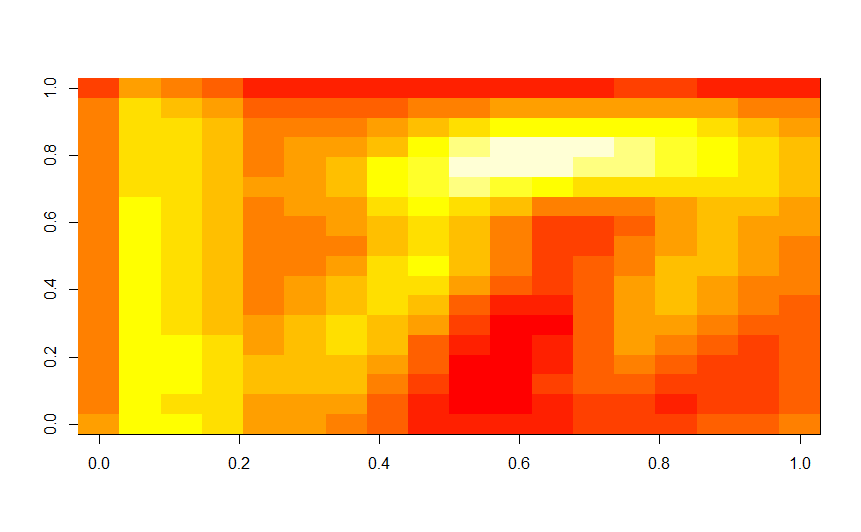
\includegraphics[width=0.49\textwidth]{eigen6.png}
        \label{fig:post}
    }\\
     \subfloat[Eigenvector 7]
    {
    	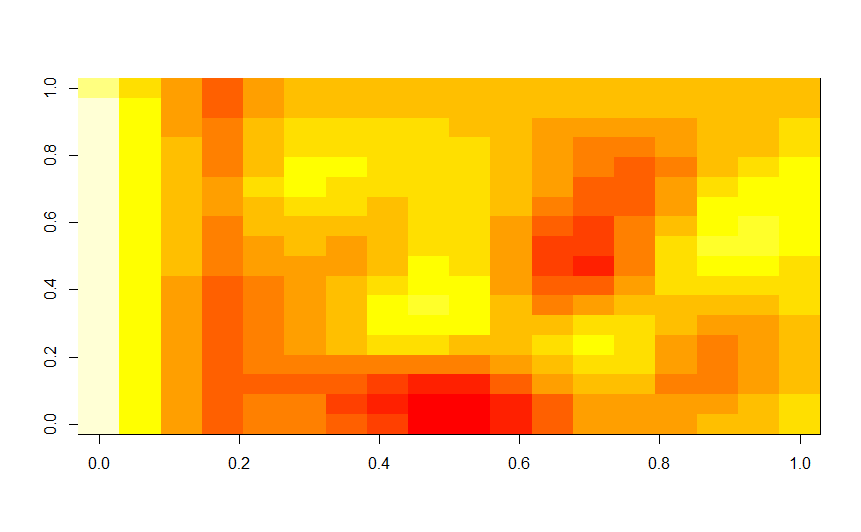
\includegraphics[width=0.49\textwidth]{eigen7.png}
        \label{fig:post}
    }
     \subfloat[Eigenvector 8]
    {
    	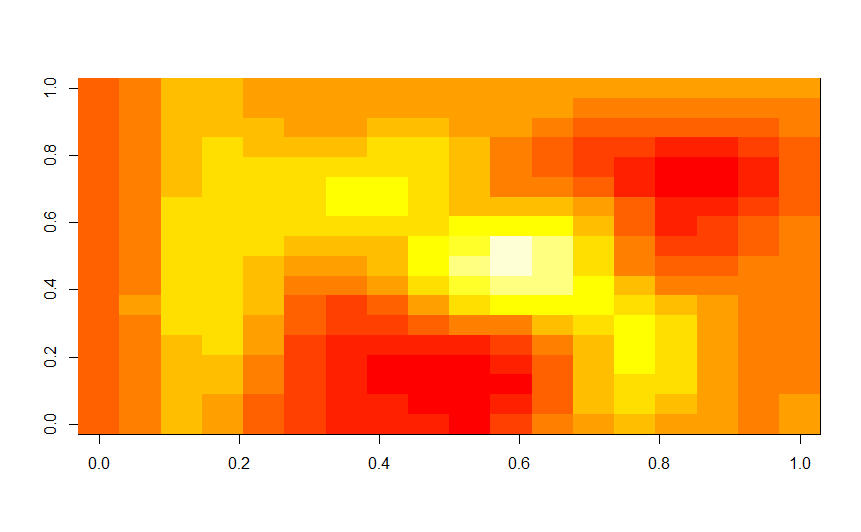
\includegraphics[width=0.49\textwidth]{eigen8.png}
        \label{fig:post}
    }\\
    \subfloat[Eigenvector 9]
	{
        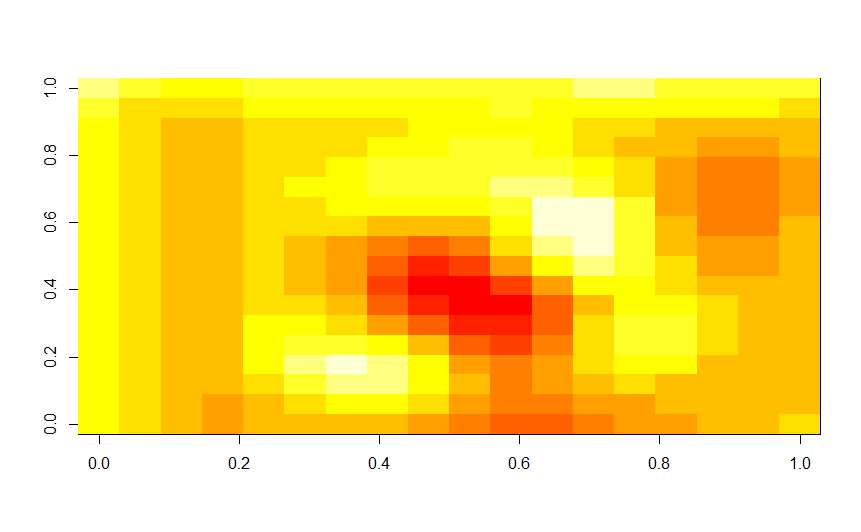
\includegraphics[width=0.49\textwidth]{eigen9.png}
        \label{fig:pre}
	}
	\subfloat[Eigenvector 10]
	{
        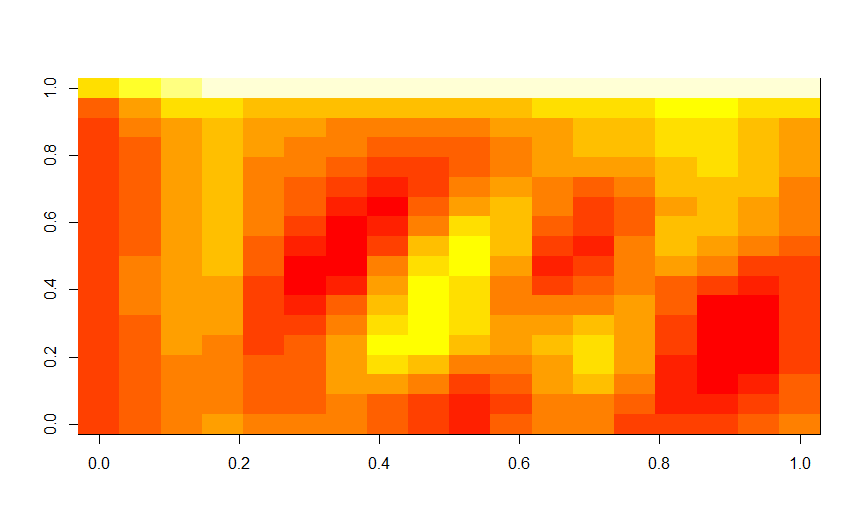
\includegraphics[width=0.49\textwidth]{eigen10.png}
        \label{fig:post}
    }
    \caption{Eigenvectors.}
    \label{fig:hist}
\end{figure}
\clearpage
\begin{figure}[h]
    \centering
    \subfloat[Reconstruction]
	{
        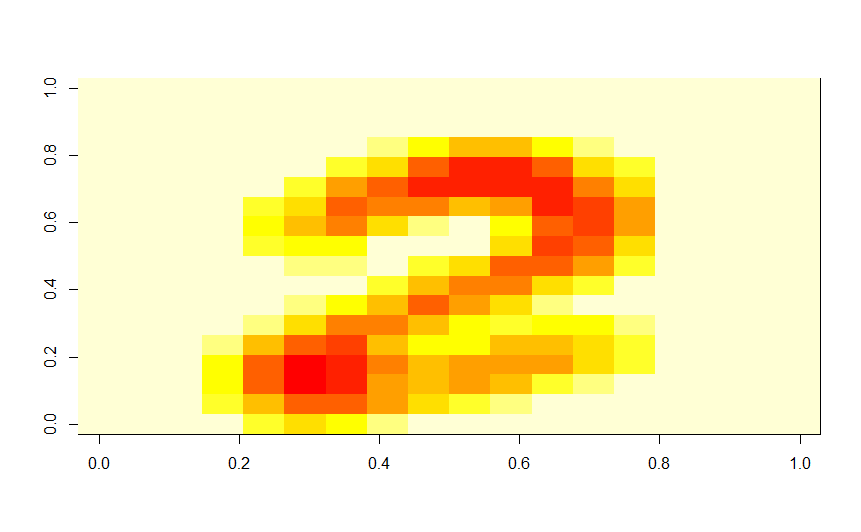
\includegraphics[width=0.49\textwidth]{recon1.png}
        \label{fig:pre}
	}
    \caption{Reconstruction with all PC's}
    \label{fig:reconFull}
\end{figure}

\subsection{Reconstruction with all PC's}
What we can see in figure \ref{fig:reconFull} is a reconstruction of one Cipher based on the eigenvectors that were created when we used the PCA algorithm, this one is made using all the Principal Components which is why it really resembles the original ones.

\subsection{Reconstruction with 80\%, 90\% and 95\% of variance}
As we know the first Principal components are the ones that have the highest variance which means that the first Principal component has the most variance and the second one has the second highest variance and so on so to achieve 80\%, 90\% and 95\% we will only need to use a fraction of the percentages in this case 19, 30 and 43 respectively.\\\\
As we can see we still get something similar as the original cipher in all of the cases but we can also see that there is a huge improvement with higher variance and although 90\% looks almost the same as the one that is using all the Principal Components it's still not as good and we get a better result when we use all of them.
\clearpage
\begin{figure}[h]
    \centering
    \subfloat[80\%]
	{
        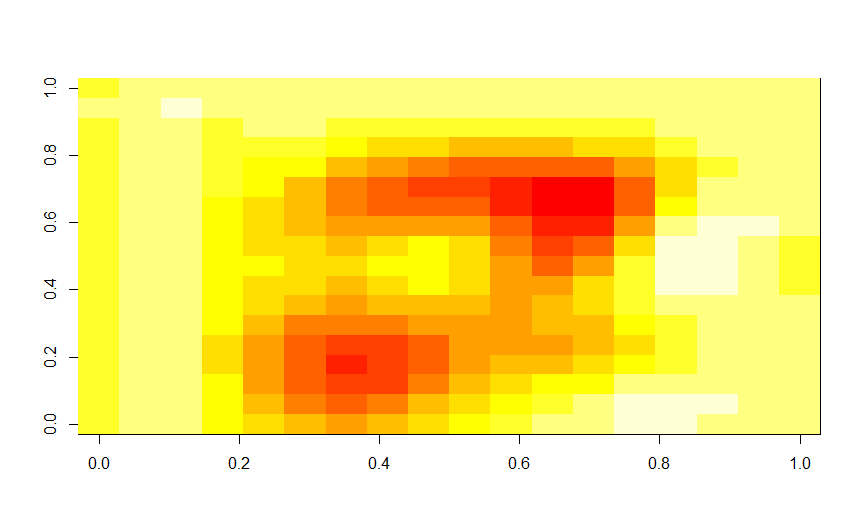
\includegraphics[width=0.49\textwidth]{recon80.png}
        \label{fig:pre}
	}
	\subfloat[90\%]
	{
        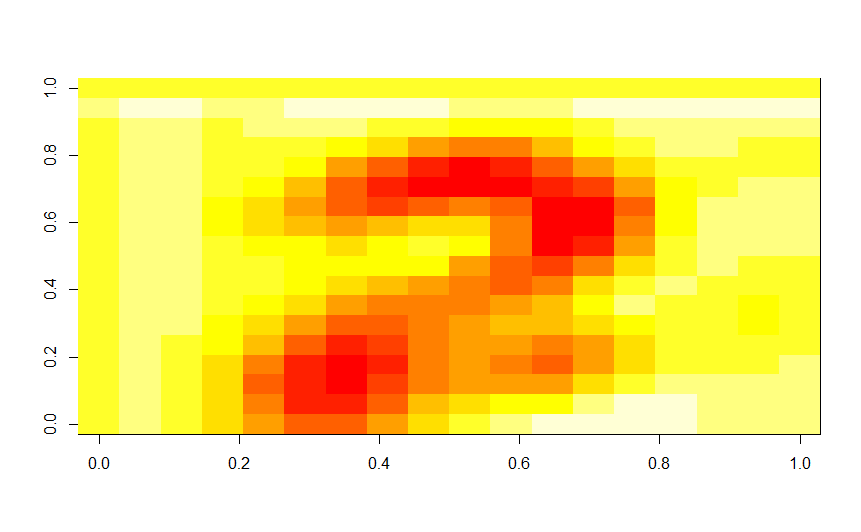
\includegraphics[width=0.49\textwidth]{recon90.png}
        \label{fig:pre}
	}\\
	\subfloat[95\%]
	{
        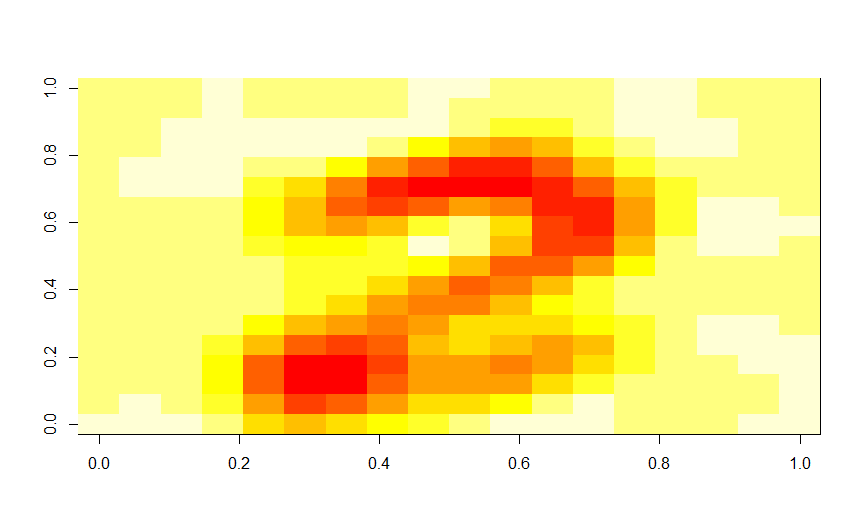
\includegraphics[width=0.49\textwidth]{recon95.png}
        \label{fig:pre}
	}
    \caption{Reconstruction with different variances}
    \label{fig:recon}
\end{figure}
\subsection{Compare 10 first scores}
In figure \ref{fig:score} we can see two different reconstructions of ciphers but only using it's first 10 scores and we can see that although it's hard to tell what original cipher they're supposed to be they still manage to look differently between them so you can see there is actually quite a difference. And as we can see in the table were we have the first 10 scores we see that although some of them are similar there are also some that have a huge difference.
\begin{table}
\begin{tabular}{|c|r|r|r|r|r|r|r|r|r|r|}
\hline
PC\ & 1 & 2 & 3 & 4 & 5 & 6 & 7 & 8 & 9 & 10 \\ \hline
1    & -0.0062  & -0.0252  & 0.08513  & -0.01152 & 0.1068 & -0.03209 & 0.07201 & -0.0396 & 0.0802 & 0.06937       \\
2    & -0.0069 & -0.03585 & 0.0799 & -0.01319 &0.08456 & 0.00585 & 0.0911 & -0.0448 & 0.0517 & -0.02189          \\ \hline
\end{tabular}
\end{table}
\clearpage

\begin{figure}[h]
    \centering
    \subfloat[First Cipher]
	{
        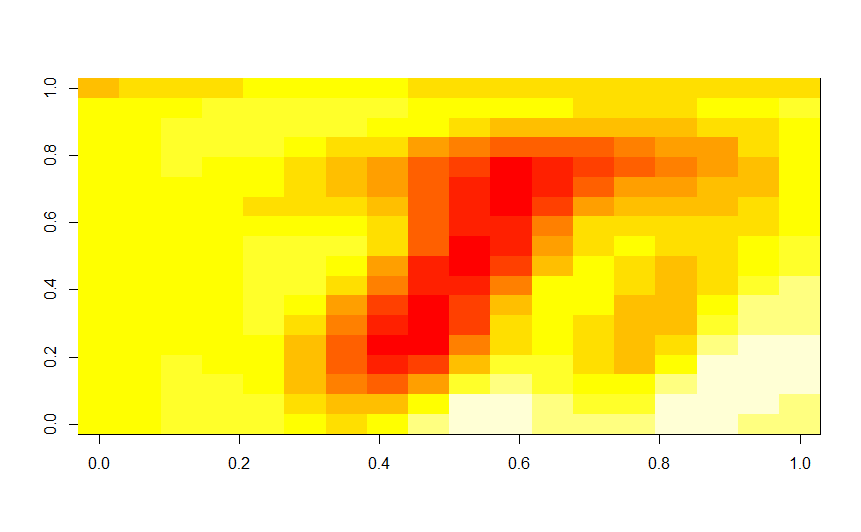
\includegraphics[width=0.49\textwidth]{10score1.png}
        \label{fig:pre}
	}
	\subfloat[Second Cipher]
	{
        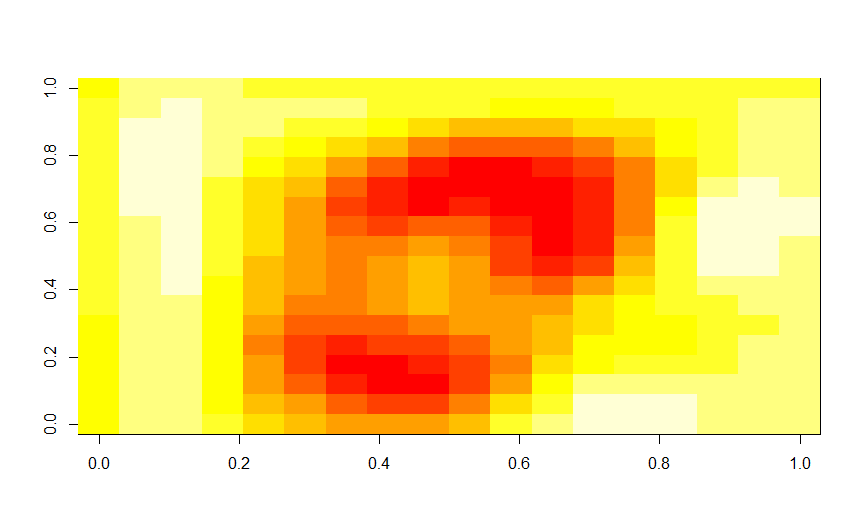
\includegraphics[width=0.49\textwidth]{10score2.png}
        \label{fig:pre}
    }
    \caption{Comparison of first scores in two ciphers}
    \label{fig:score}
\end{figure}

%>>>>>>> 356a59bae290031cdbac0b8bf5fb29f42330ad28

%We will be using R which is a statistical language in order to test the k-nearest neighbor algorithm, firstly we will have to generate our data-sets which are taken from scanned ciphers and loaded through the function \texttt{loadSinglePersonsData}, once the data is loaded we shuffle the data with a seed for reproducible results. With this done we split the data into test and train so that we are able to test the data after we have trained and be able to use different data from the one that was trained.



\begin{flushleft}
%For this test we will be varying the number of k to see how the result actually varies when we begin to change it's value we will check how the speed and test recognition are affected by this change. This is to see how important really is to select the correct k and to see if having selected the wrong one could affect your results substantially.
\end{flushleft}

\begin{flushleft}
%We will also be doing cross validation of the results in order to see if the results of the trained model will fit for other hypothetical, set of data this will be done by running 10 times a 90\%/10\% split of the data-set. The pseudocode for the cross-validation is shown below.
\end{flushleft}

\begin{flushleft}
%Finally after testing it with the smoothing implementation that was in \texttt{loadImage.r} we have to implement the smoothing using a different method. We used the Gaussian smoothing  with various sigmas, this is implemented in the EBImage package as \texttt{gblur()} which receives as parameter the image and the sigma.   
\end{flushleft}
%------------------------------------------------


%----------------------------------------------------------------------------------------


%We see that the accuracy does vary with k. Notably, k=1 results in a perfect fit for the training set but this will often, in theory, result in overfitting of the data. Thus we use the rule of thumb of taking the square root of the sample size as the k and approximate it to k=50 for further testing.\\

%Though the timing measurements presented in the table are quite noisy, we see that the computation time seems to increase with DPI. This is logical as the number of pixels in the images has a square relationship to the DPI. Below we will present more accurate timing measurements and discuss their dependence on k.\\

%For more accurate timing measurements, we ran the \texttt{knn()} function repeatedly for k=1 and k=100 and compared the results. for DPI=300, we obtained mean computation times of 3.98s and 4.75s for k=1 and k=100, respectively. This is to be expected as for larger k, each point needs to be checked against more neighbours, resulting in more computations.\\

%We performed cross-validation on the data with our chosen k for varying DPI values. In general, we found the accuracy of the kNN algorithm to be independent on the image quality, at least for the DPI values tested. Thus only results for DPI=100 are shown below. We obtained a mean accuracy of 0.880 with a standard deviation of 0.056.\\


%For our tests with image preprocessing we obtained the results shown below for different sigmas in the gaussian low-pass smoothing filter. We see that the smoothing seems to increase the accuracy of the algorithm to some degree.\\


%Finally we ran the first test on the entire data set. Cross-validation as well as accurate timing was not performed for this part due to a lack of computation power. This was also the reason we only tested with k=50. k=200 may have been more accurate as the data set was 18 times larger than in previous parts.\\

%We obtained accuracy results of 0.9954 on the training set and 0.9949 on the test set. We timed the execution time of the \texttt{knn()} function and found it to be 20 minutes and 35 seconds. From these results, in comparison to the previous, one can argue that the benefit of having a larger data set is greater than the variance introduced by different handwritings. Moreover, the variance in handwriting in the data may even be beneficial to the accuracy of the algorithm.\\



%--------------------------------------------------

\end{document}
\grid
